\documentclass{article}

% The geometry package allows for easy page formatting.
\usepackage{geometry}
\geometry{letterpaper}

% Load up special logo commands.
\usepackage{doc}

% Package for formatting URLs.
\usepackage{url}

% Packages and definitions for graphics files.
\usepackage{graphicx}
\usepackage{epstopdf}
\usepackage{natbib}
\usepackage{tikz}
\DeclareGraphicsRule{.tif}{png}{.png}{`convert #1 `dirname #1`/`basename #1 .tif`.png}

%
% Set the title, author, and date.
%
\title{Panthera: A Study of Caching in Distributed Computing}
\author{Dhaivat Pandya \\ Appleton North High School}
\date{}
%
% The document proper.
%
\begin{document}

% Add the title section.
\maketitle

% Add an abstract.
\abstract{
The adoption of distributed computing systems has grown massively in the past few years. In particular, Apache Hadoop, which allows developers to create applications that run on a cluster of computers, is currently used throughout academia and industry. However, the Hadoop File System fails to effectively utilize memory and local storage in order to reduce waiting time (i.e. latency). In this project, a system, named Panthera, was developed, which creates a caching system for Hadoop metadata and data. Panthera caches both information about files and the file contents, thereby reducing waiting time in downloading and accessing the files and related information. It runs with an unmodified version of Hadoop, meaning that it can integrate easily into existing architecture. Panthera was tested using both single node and multi-
node setups. The results showed an 90.8\% decrease in waiting time with the Panthera metadata cache, and a 95.7\% decrease with the Panthera data cache. Such drastic decreases in latency can greatly increase the efficiency of existing Hadoop applications and also allow the creation of algorithms that were previously not feasible. Panthera has numerous applications in fields ranging from market research to bioinformatics. All code associated with the project will be open sourced to further development in the area.
}

\section{Introduction}
Distributed computing systems are currently employed across academia and industry. Applications vary from market research for department stores to bioinformatics. In particular, the Hadoop distributed system \cite{hadoop} has seen tremendous growth. Hadoop is an open source version of the revolutionary MapReduce system developed at Google. With it, developers can take easily take advantage of large, multi-node clusters to solve computational problems.

Current Hadoop deployments exist in the thousands of nodes at companies such as Cloudera, Facebook, Yahoo, etc. However, especially in larger networks, file access latency can be a significant. The Hadoop File System currently does not use local (i.e. on the client) random access memory (RAM) to improve latency.

Latency in distributed systems can have significant effects, and a reduction of the same comes with tremendous benefits. As the RAMCloud project has outlined \cite{ramcloud}, low latency can greatly extend the applications of distributed computing systems. For example, tree traversal algorithms are largely impractical in Hadoop, however, with lower latency, such algorithms may become useful and applicable.

In this paper, we discuss \textit{Panthera}, a cache layer for Hadoop. In Section 2, we discuss the specific challenges associated with such a project. Section 3 details the architecture differences between a standard Hadoop installation and one with \textit{Panthera}. 

\section{Constraints}

There are several systems built on Hadoop that are in widespread use \cite{hbase, cloudbatch, pig}. The Hadoop project is also supported by large corporations with a 
consistent release cycle. Thus, for \textit{Panthera} to be practical, it must operate independently of the existing Hadoop codebase, i.e. as a layer, rather than a modification. This implies that \textit{Panthera} is implemented completely independently of the Hadoop codebase.

Additionally, for non-cache related requests, \textit{Panthera} must add insignificant latency. Finally, data and metadata request latency should be significantly with \textit{Panthera} in comparison to a standard Hadoop installation.

\section{Architecture}
\begin{figure}[!h]
  \caption{Standard Hadoop Architecture (left), Panthera-Hadoop Architecture (right)}
  \centering
	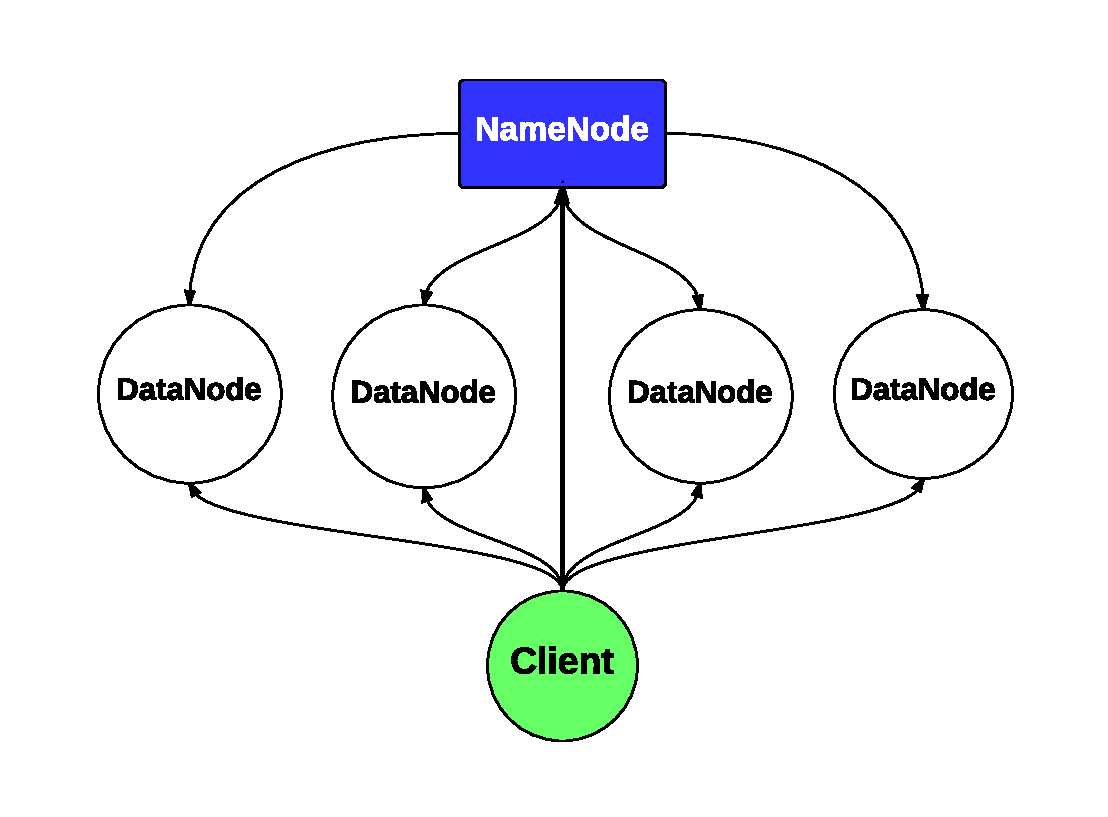
\includegraphics[scale=0.4]{assets/hadoop_architecture.pdf}
	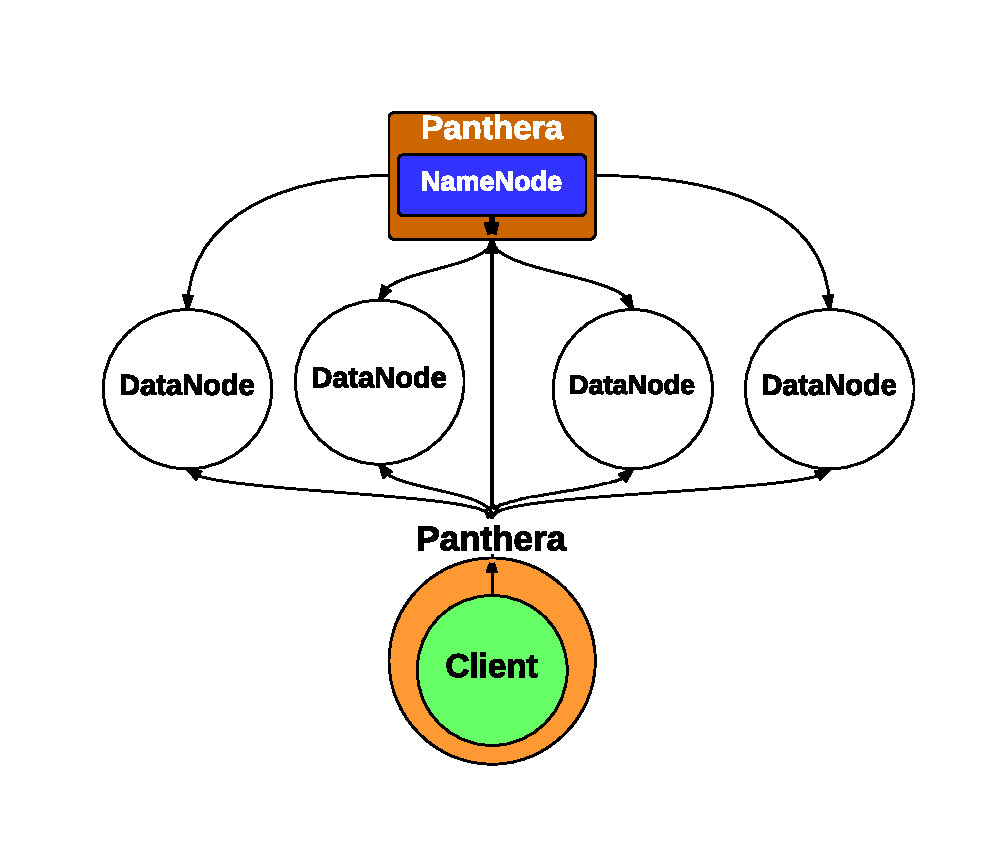
\includegraphics[scale=0.4]{assets/panthera_architecture.pdf}
\end{figure}

Figure 1 outlines the architecture differences between a standard Hadoop File System architecture and an installation with Panthera. 

Within the standard conditions, the \textit{NameNode} serves as a metadata server, handling all requests from clients relating to metadata (e.g. directory listing, file sizes, block locations, etc.). \textit{DataNode(s)} hold data and serve it at request from the client. A more complete description of the Hadoop File System may be found in \cite{hadoop}.

Panthera operates by intercepting requests and responses at the NameNode and the client. Both nodes have a running instance of \textit{Panthera}. Every request issued from the client is first reviewed by Panthera, and if possible, answered immediately from the cache. The \textit{Panthera} instance on the NameNode constantly monitors the filesystem for changes that need to be reflected in the cache (e.g. if a file is deleted, the cache on the client should have a copy of it).

Panthera, since it caches both data and metadata, can be considered two separate subsystems, which are now discussed.

\section{Metadata caching}

\begin{figure}[!h]
	\caption{Panthera Metadata System}
	\centering
		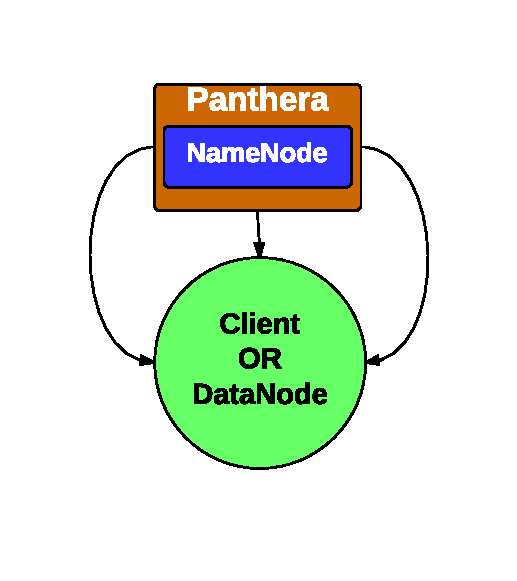
\includegraphics[scale=0.4]{assets/panthera_meta_architecture.pdf}
\end{figure}

The Panthera metadata system runs on the NameNode and communicates with the Panthera instance on the client. The challenge on the metadata portion consist of reducing computational latency to memory latency. For example, for some intensive methods (e.g. a recursive directory listing), it may be worthwhile to cache a response in order to prevent computing the same list again.

However, the problem lies in identifying such methods. Obviously, there are some methods for which caching is not worthwhile since their execution time is lower or comparable to memory latency. Within Panthera, six different Hadoop query methods were identified as medium to high latency. Panthera identifies packets that contain these methods and subsequently caches them.

Currently, a standard LRU cache is used for each method. Testing of different caching methods and predictive prefetching algorithms is under way.

\section{Data caching}

\begin{figure}[!h]
	\caption{Panthera Data System}
	\centering
		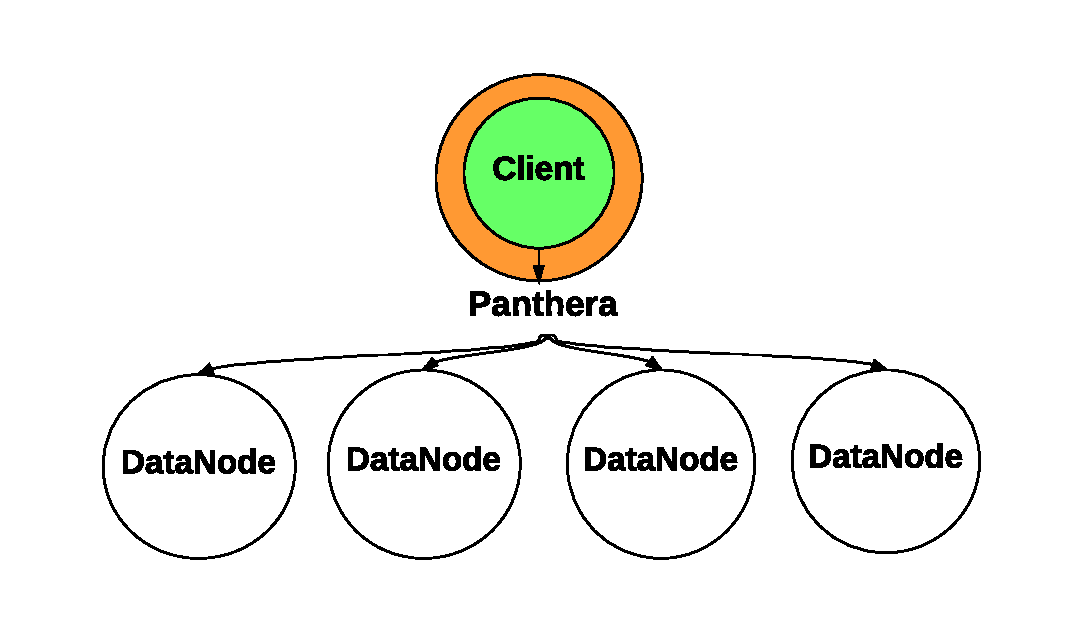
\includegraphics[scale=0.4]{assets/panthera_data_architecture.pdf}
\end{figure}

Panthera's data caching system runs on the client. The architecture is similar to that of the metadata caching system. Every request that the client makes to the DataNodes is first processed by Panthera and responded to from the cache if possible. 

The challenges with data caching differ significantly from those in metadata caching. Here, the goal is to convert network and hard drive read latency into memory latency. As \cite{ramcloud, hadoop} note, memory latency can be extremely low in modern systems, especially in comparison to network and hard drive latencies. Thus, in some respects, the goal is "easier" to attain in the data cache. However, for smaller files, it may be difficult to obtain latency improvement. 


\section{Testing Methodology}

In testing Panthera, very simple strategies were adopted. In order to test the metadata cache, a directory listing query was repeatedly run on a directory with 100 files in it, and the latency times for responding are measured, with Panthera and without. The reasoning for picking such a test lies in the fact that a directory listing in Hadoop involves all six of the cached methods as well as a few non-cached methods. Thus, the test provides a good estimate of the efficacy of the cache.

Latency times for the data cache were obtained by repeatedly querying for a one megabyte large file. The test encapsulates the most common use case for Panthera and the Hadoop File System.

Tests for the metadata cache were conducted on both single node and multinode setups, whereas the datanode cache testing was run on multinode setups.

\section{Results: Data caching}
\begin{figure}[!h]
	\caption{Panthera data cache latencies}
	\centering
		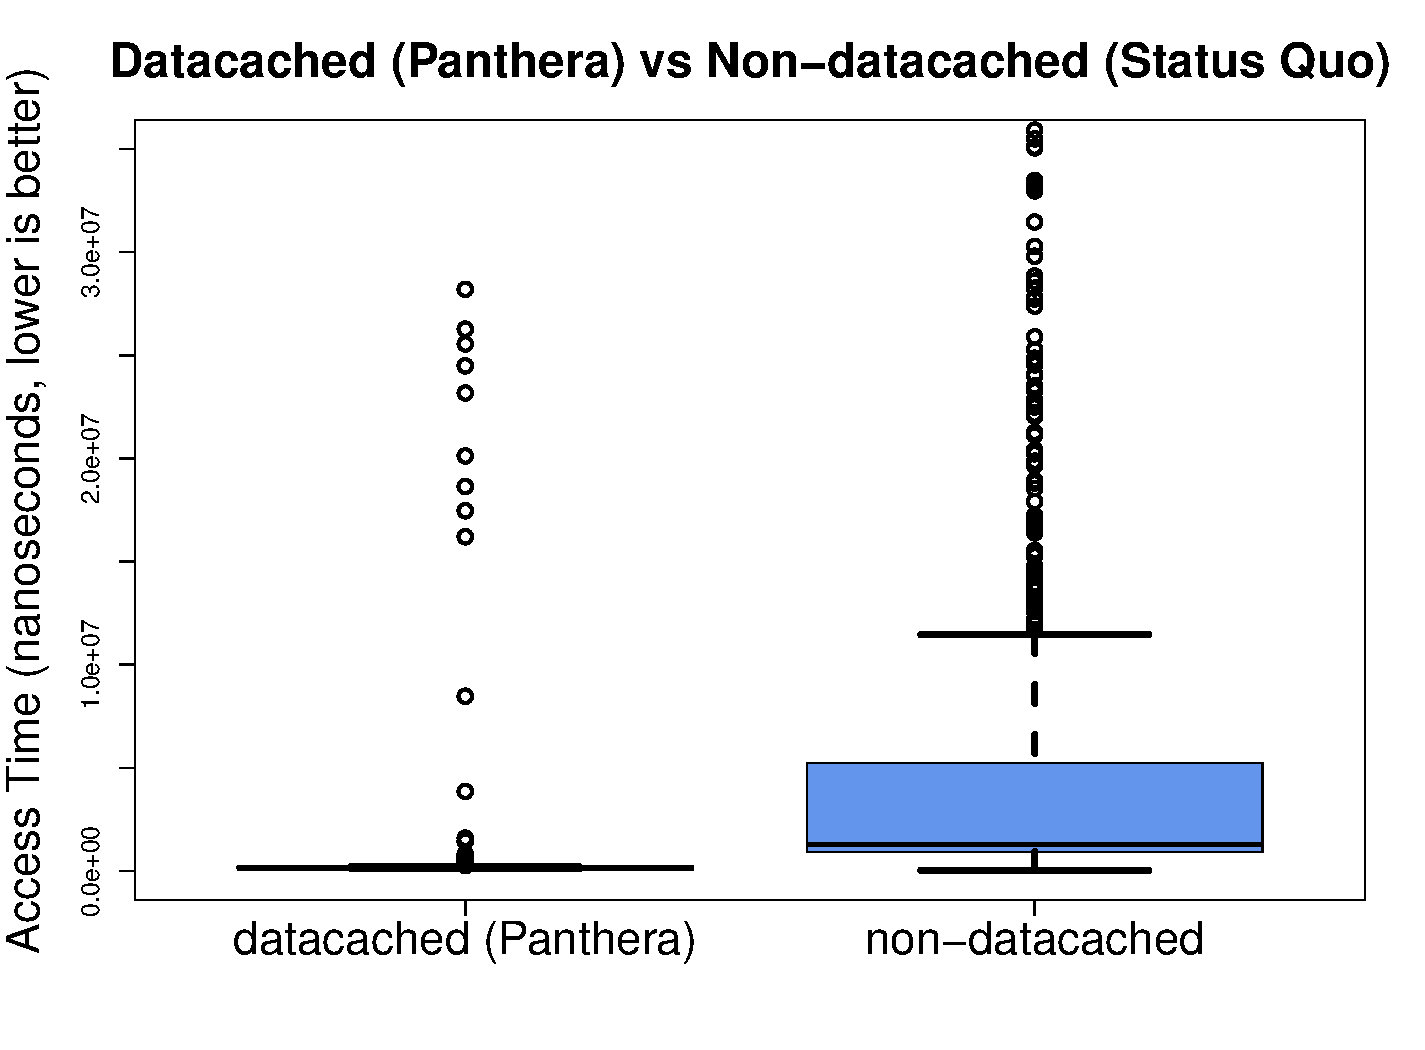
\includegraphics[scale=0.4]{assets/box-plot-data.pdf}
\end{figure}

The Panthera data cache showed a 95.7\% decrease in the latency in comparison to a standard deviation non-datacached installation. In addition, the standard of deviation was lower by a factor of 27. For any deployed project, maximum levels of latency must be considered when designing a system. Thus, the \textit{status quo} of the non-cached version severely limits possibilities within Hadoop.

\section{Results: Metadata caching}
\begin{figure}[!h]
	\caption{Panthera metadata cache latencies}
	\centering
		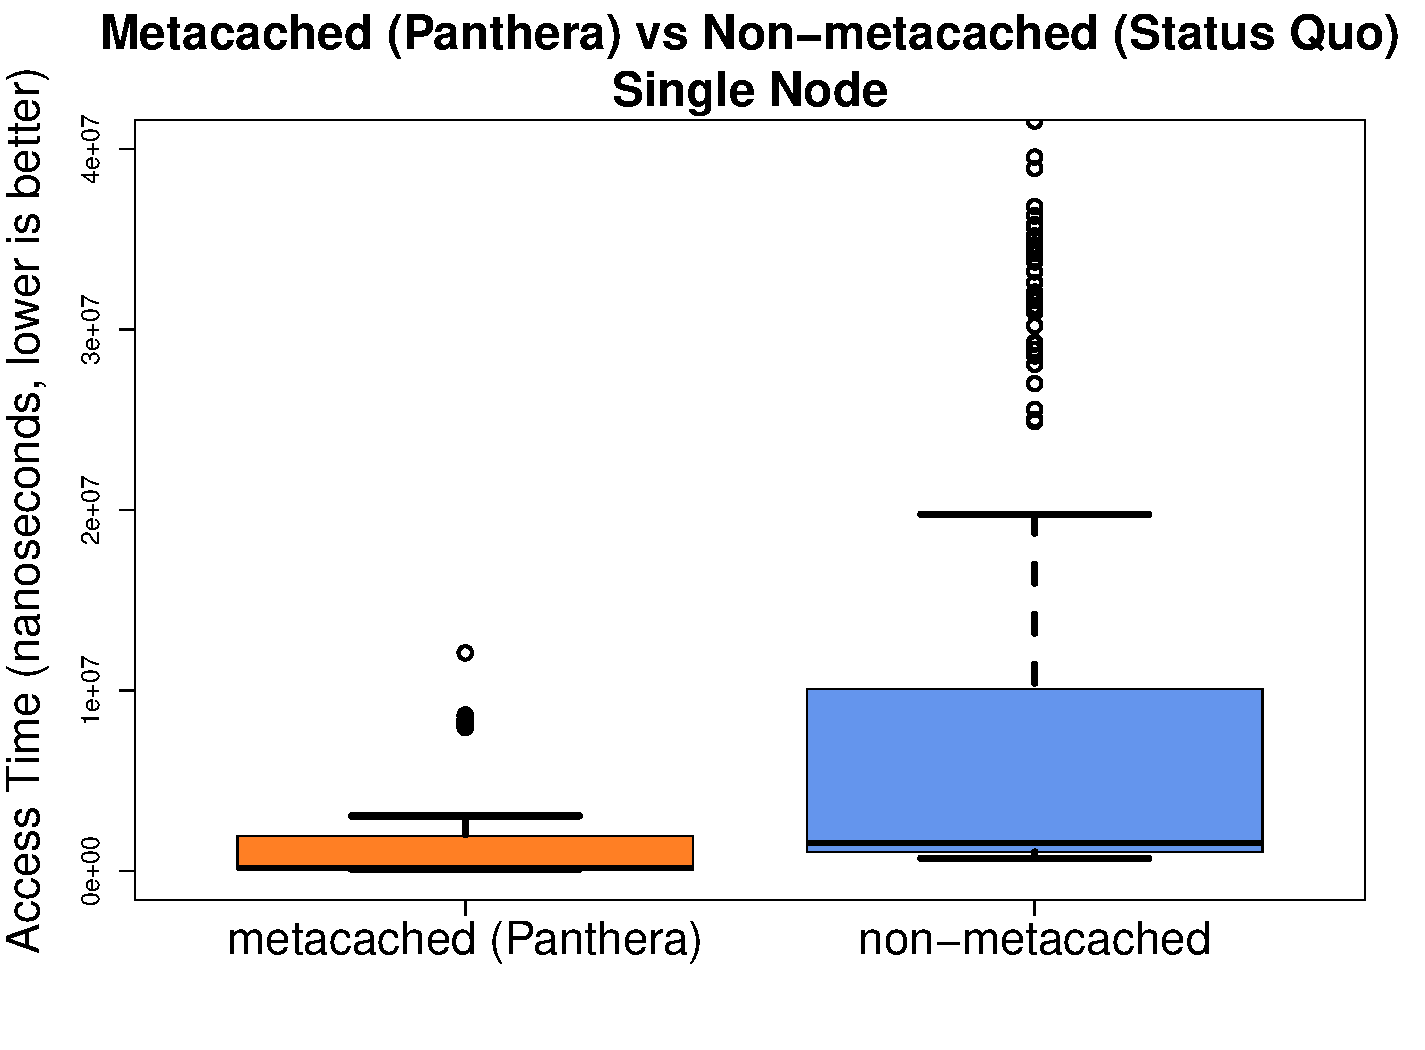
\includegraphics[scale=0.3]{assets/box-plot-metadata.pdf}
		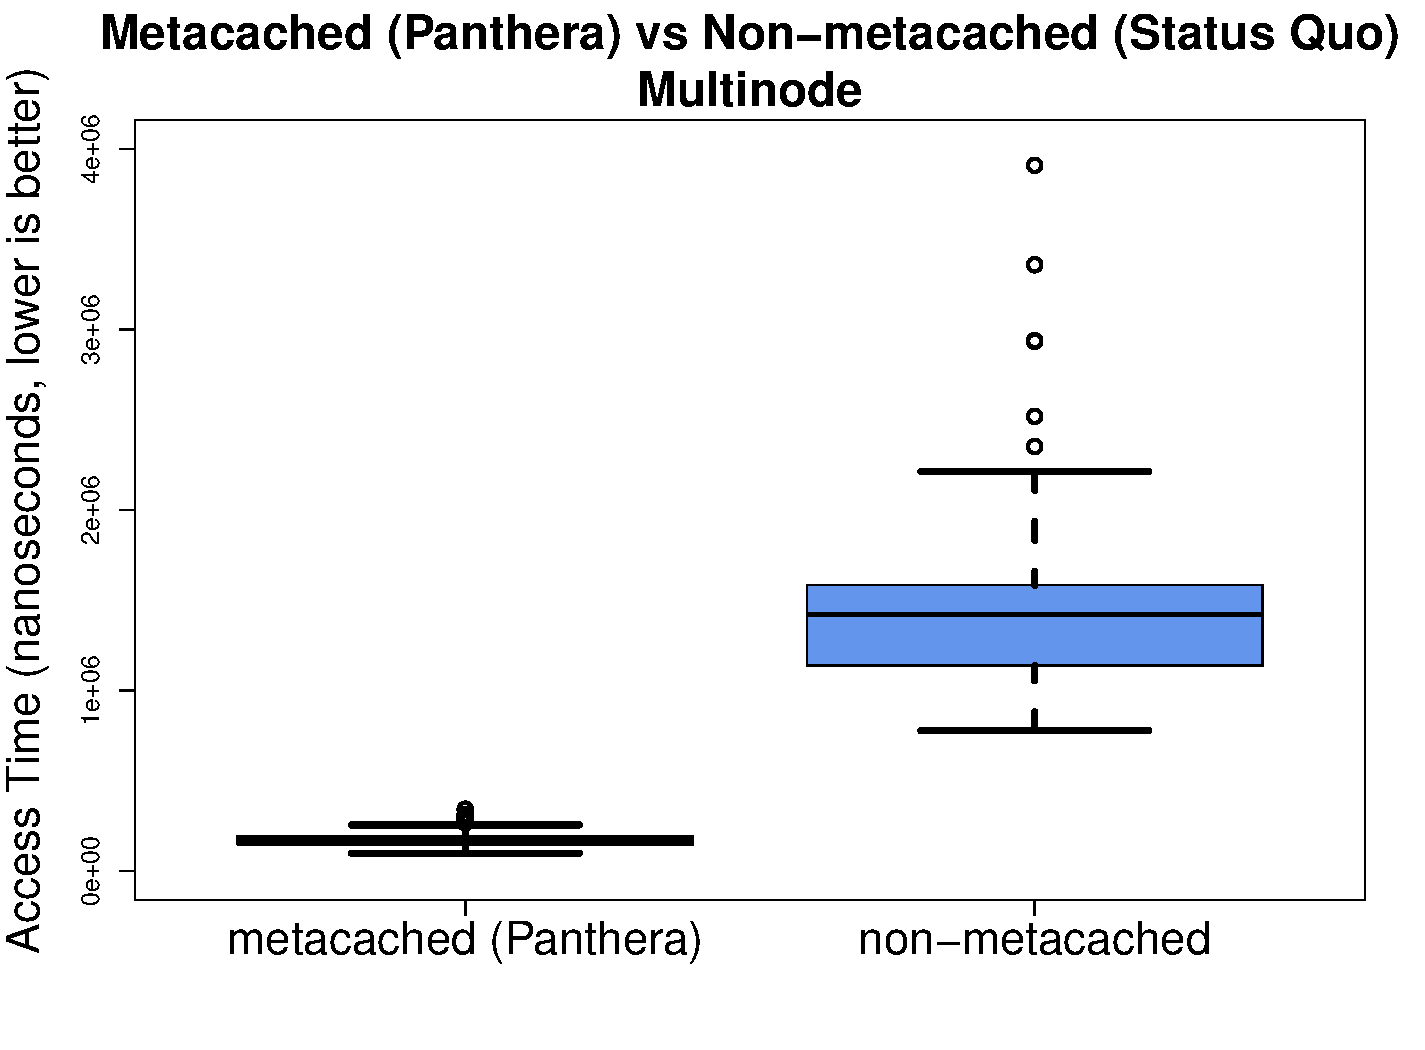
\includegraphics[scale=0.3]{assets/box-plot-metadata-multinode.pdf}
\end{figure}

Metadata caching has similarly incredible results. \textit{Panthera} showed a 9 fold or 90.8\% improvement in the total latency as measured on the client side in a multinode setup. Additionally, the standard deviation is 24 fold lower in \textit{Panthera}.

\section{Conclusion}

\textit{Panthera} fulfils the constraints mentioned at the outset. It is a layer on Hadoop rather than a main repository code modification. Considering the latency measurements, it is clear that it has also met the requirements in terms of benefit. \textit{Panthera} was able to reduce data access latency by 95.7\% and reduce basic metadata access latency by 90.8\%. Additionally, \textit{Panthera} greatly reduced the variation in the access latency, greatly aiding in the pre-development plans and extending the capabilities of distributed computing systems such as Hadoop.

\section{Future work}
\textit{Panthera} can be extremely useful in a wide variety of applications, specifically in those which require large datasets in separate files (e.g. unstructured data). In particular, I will be concentrating on bioinformatics and integrating Panthera's caching with algorithms used in the area.

I am also working on a cache-based scheduler for Hadoop. Essentially, it will use information about what files are available in various clients and arrange Hadoop tasks such that the use of the cache is maximized.

Finally, all code associated with this paper and \textit{Panthera} will be open sourced in order to further development of Hadoop and distributed computing.

\nocite{*}

\bibliographystyle{plain}
\bibliography{references}

\end{document}